\section{Evaluation}\raggedbottom
Im nachfolgenden Kapitel sollen nun die Ergebnisse der praktischen Anwendung der Klassifikationstechniken auf die vorliegenden Datensätze ausgewertet werden. Wie in den vorangegangenen Kapiteln besprochen, wird erwartet, dass verschiedene Techniken der Merkmalsextraktion, verschiedene Level der Dimensionalitätsreduktion und verschiedene Hyperparametereinstellungen die Ergebnisse qualitativ beeinflussen werden. Eine in dieser Arbeit angewandte Methode, die es ermöglicht, diese Unterschiede zu messen und gleichzeitig die beste Kombination zu bestimmen, ist die sogenannte Hyperparameteroptimierung. Hierbei wird das gewählte Verfahren wiederholt mit unterschiedlichen, zuvor gewählten Parameterkombinationen auf den Merkmalraum angewandt. Nach der Besprechung jener Optimierungsergebnisse im Einzelnen, sollen die Perfomances der Verfahren abschließend noch in einen Gesamtzusammenhang gestellt und verglichen werden.
\subsection{Implementierung} 
Zwecks Nachvollziehbarkeit und Transparenz soll an dieser Stelle kurz auf die parallel erfolgte praktische Anwendung der beschriebenen Techniken eingegangen werden.\\
Im Rahmen dieser Abschlussarbeit wurde ein Kommandozeilen-Tool namens \glqq TrollDetector\grqq{} \footnote{\url{https://github.com/rokoe102/trolldetector}} in der Programmiersprache Python entwickelt. Dieses hat mehrere Funktionen. Zum einen ist damit möglich, ein beliebiges Klassifikationsverfahren mit selbst gewählten Hyperparametern auf den Datensatz anzuwenden. Dies geschieht nach dem bereits erwähnten \glqq Train-and-Test\grqq-Verfahren. Hier sind auch Merkmalsextraktion (z.B. TF vs. TF-IDF) und Dimensionalitätsreduktion direkt steuerbar.\\
Eine weitere Funktion ist die Hyperparameteroptimierung für jedes Verfahren mit anschließender Auswertung der Ergebnisse. Für die Optimierung wird eine Rastersuche verwendet. Bei dieser Methode wird das jeweilige Klassifikationsverfahren auf einer fest definierten Untermenge aller möglichen Kombinationen von Hyperparametern ausgeführt. Anschließend werden die Ergebnisse der Kombinationen ausgewertet.\\
Schließlich ist es mit dem Programm noch möglich, einen Vergleich der fünf Klassifikatoren anzustellen. Die voreingestellten Hyperparameter sind jene, welche bei der Hyperparameteroptimierung am besten abgeschnitten haben, sodass eine Vergleichbarkeit hergestellt wird.\\
Zur Verarbeitung und Klassifikation des Datensatzes wurden ausschließlich Klassen und Funktionen aus der \glqq scikit-learn\grqq-Bibliothek von \citet{scikit-learn} verwendet.\\
\pagebreak
\subsection{Erklärte Varianz}
Ein Hyperparameter, der grundsätzlich auch in der Rastersuche mit berücksichtigt werden kann, ist das Level der Dimensionalitäsreduktion. Dies bringt jedoch einen fundamentalen Konflikt mit sich: Das Testen von mehreren Werten für die Dimensionen würde gleichsam ein Vielfaches an Ausführungen und damit eine deutlich gesteigerte Laufzeit mit sich bringen. Andererseits liefern mehr Vektorkomponenten auch mehr Informationsgehalt (eine größere Varianz) und damit bessere Ergebnisse, die auch interessant für die Optimierung sind. Letztere Proportionalität ermöglicht aber auch eine alternative Vorgehensweise: Man kann das Reduktionslevel $d$ für alle Ausführungen konstant wählen. In diesem Fall ist es entscheidend, ein $d$ zu wählen, was den Anforderungen der Laufzeit und der Qualität gerecht werden kann. Wie in Kapitel \ref{dim-red} beschrieben, kann der Informationsgehalt der einzelnen Vektorkomponenten im Zuge einer Hauptkomponentenanalyse oder einer Singulärwertzerlegung ermittelt werden. Man spricht hier von der durch eine Komponente \textbf{erklärten Varianz}.
\begin{figure}[htb]
	\begin{center}
		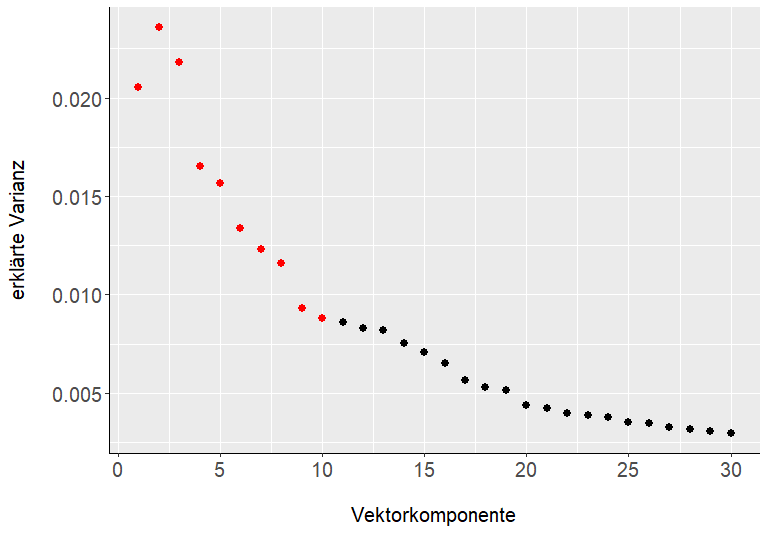
\includegraphics[width=0.95\textwidth]{bilder/expvar.png}
		\caption{Erklärte Varianz der Komponenten}\label{expvar}
	\end{center}
\end{figure}\\
Abbildung \ref{expvar} zeigt nun die 30 höchsten Werte der erklärten Varianz nach einer Singulärwertzerlegung der Vektoren des Datensatzes. Demnach erklären 3 Komponenten über 2\% der Varianz, 5 Komponenten zwischen 2 und 1\% der Varianz und der Rest die übrige Varianz. Kumuliert man diese Werte, werden durch die besten 10 Komponenten (rot) 15\% der Varianz erklärt. Dies ist für die geringe Anzahl der Komponenten ein vertretbarer Informationsgehalt. Da $d = 10$ gleichzeitig ebenfalls laufzeitverträglich ist, wird dieser Wert konstant für alle nachfolgenden Anwendungen gewählt.
\pagebreak
\subsection{Hyperparameteroptimierungen}
Zu Beginn soll jedes Verfahren einzeln auf die Eignung als Trollerkennungsinstrument untersucht werden. Hierzu werden die Ergebnisse der Hyperparameteroptimierungen diskutiert. Folgende Hyperparameter teilen sich dabei alle Verfahren, da die Merkmalsextraktion bei ihnen gleich abläuft:
\begin{table}[htb]
	\begin{center}
		\begin{tabular}{|c|c|}
			\hline
			Hyperparameter & gewählte Werte \\ \hline \hline
			Merkmalgewichtung & TF, TF-IDF \\ \hline
			Stoppwort-Filterung & keine, englisch\\ \hline
			n-Gramm-Extraktion & 1-Gramme, 1+2-Gramme\\ \hline			
		\end{tabular}
		\caption{gemeinsame Hyperparameter aller Verfahren}\label{common-params}
	\end{center}
\end{table}\\
Alle anderen Parameter sind verfahrensspezifisch.
\subsubsection{k-Nearest-Neighbor-Algorithmus}
Beim KNN-Algorithmus sind neben den Hyperparametern, welche mit anderen Verfahren geteilt werden, die Abstandsmetrik und der k-Wert für die zu untersuchenden Nachbarn gegeben.\\
Tabelle \ref{results-knn} zeigt die mittleren Ergebnisse verschiedener Ausprägungen aller Hyperparameter einerseits im Vergleich untereinander und im Vergleich zur durchschnittlichen und zur besten Performance. Hieraus lassen sich verschiedene Schlussfolgerungen ziehen:\\
\begin{table}[htb]
	\begin{center}
		\begin{tabular}{|c|c|c|c|c|c|c|}
			\hline 
			Hyperparameter & Genauigkeit & Relevanz & Segreganz & Sensitivität & Spezifität & $F_1$ \\ \hline \hline
			TF & \textbf{0.951} & \textbf{0.937} & 0.965 & 0.964 & \textbf{0.937} & \textbf{0.949} \\ \hline
			TF-IDF  & 0.949 & 0.932 & \textbf{0.966} & 0.964 & 0.935 & 0.948 \\ \hline \hline
			engl. Stoppwörter  & 0.947 & 0.931 & 0.962 & 0.961 & 0.934 & 0.946 \\ \hline
			keine Filterung  & \textbf{0.953} & \textbf{0.937} & \textbf{0.968} & \textbf{0.967} & \textbf{0.940} & \textbf{0.952} \\ \hline \hline
			1-Gramme  & \textbf{0.955} & \textbf{0.941} & \textbf{0.969} & \textbf{0.967} & \textbf{0.967} & \textbf{0.954} \\ \hline 
			1+2-Gramme  & 0.945 & 0.928 & 0.962 & 0.961 & 0.961 & 0.944 \\ \hline \hline
			$k = 5$  & \textbf{0.953} & \textbf{0.938} & \textbf{0.967} & \textbf{0.966} & \textbf{0.940} & \textbf{0.952} \\ \hline 
			$k = 15$  & 0.950  & 0.934  & 0.965  & 0.964 & 0.936  & 0.949 \\ \hline 
			$k = 25$  & 0.948  & 0.931  & 0.964  & 0.962 & 0.934  & 0.947  \\ \hline \hline
			euklid. Metr.  & 0.950 & \textbf{0.935} & 0.965 & 0.963 & 0.937 & 0.949 \\ \hline
			Manhattan  & 0.950 & 0.934 & \textbf{0.966} &\textbf{0.964} & 0.937 & 0.949 \\ \hline
			 \hline
			Maximum  & 0.960 & 0.948 & 0.973 & 0.972 & 0.950 & 0.959 \\ \hline
			durchschnittl. & 0.950 & 0.934 & 0.965 & 0.964 & 0.937 & 0.949 \\ \hline
		\end{tabular}
		\caption{Ergebnisse bei KNN}\label{results-knn}
	\end{center}
\end{table}\\\\
Insgesamt sind beim KNN-Algorithmus ausgezeichnete Zahlen zu beobachten. Im Maximum liegen  nahezu alle Kennzahlen über 95\%, positiv auffallend sind hier Werte der Segreganz und der Sensitivität von über 97\%. Durchschnittlich werden immer Punktzahlen von über 93\% erreicht. Ein Unterschied im Abschneiden unterschiedlicher Parametereinstellungen ist bei der Merkmalsgewichtung zu erkennen: TF erreicht hier ein wenig bessere Punktzahlen als TF-IDF. Die Filterung von englischen Stoppwörtern bringt im Mittel keine Verbesserung hervor. Extrahiert man nur 1-Gramme, anstatt 1-Gramme und 2-Gramme, erreicht man bis zu 1\% höhere Punktzahlen.\\
Bei den verfahrensspezifischen Hyperparametern gibt es nur wenige Schwankungen. Beim k-Wert deutet sich an, dass ein einstelliger Wert besser abschneidet als ein zweistelliger, die Verbesserungen belaufen sich aber nur auf höchstens 0,5\%. Bei den Metriken ist auffällig, dass unterschiedliche Arten der Abstandsmessungen nahezu keinen Unterschied in der Qualität hervorbringen, die Abweichungen betragen hier höchstens 0,1\%.\\
Angesichts seiner durchweg hohen Punktzahlen in allen möglichen Gütemaßen ist der k-Nearest-Neighbor-Algorithmus sehr gut für die Erkennung von IRA-ähnlichen Trollen geeignet.
\subsubsection{Naiver Bayes-Klassifikator}
Der einzige verfahrensspezifische Hyperparameter des Naiven Bayes-Klassifikators ist die angenommene Verteilung der Merkmalvektoren. Getestet wurde mit einer Normalverteilung, einer Multinomialverteilung und einer komplementären Verteilung nach >Rennie et al. (2003)<.\\
Die Ergebnisse in Tabelle \ref{results-nb} lassen folgende Schlüsse zu:\\
Dieses Verfahren schneidet je nach Parameter-Einstellung sehr unterschiedlich ab. So liefert die Annahme einer Normalverteilung oder einer komplementären Verteilung Punktzahlen von 75 - 85\%.
\begin{table}[htb]
	\begin{center}
		\begin{tabular}{|c|c|c|c|c|c|c|}
			\hline 
			Hyperparameter & Genauigkeit & Relevanz & Segreganz & Sensitivität & Spezifität & $F_1$ \\ \hline \hline
			TF         & \textbf{0.747} & 0.772 & \textbf{0.767} & \textbf{0.685} & 0.804 & \textbf{0.694} \\ \hline
			TF-IDF     & 0.702 & \textbf{0.798} & 0.736 & 0.571 & \textbf{0.824} & 0.536 \\ \hline \hline
			engl. Stoppwörter  & 0.715 & 0.751 & 0.731 & 0.620 & 0.803 & \textbf{0.616} \\ \hline
			keine Filterung    & \textbf{0.734} & \textbf{0.819} & \textbf{0.77}1 & \textbf{0.636} & \textbf{0.825} & 0.614 \\ \hline \hline
			1-Gramme    & 0.735 & 0.811 & 0.761 & 0.642 & 0.642 & 0.631 \\ \hline 
			1+2-Gramme  & 0.713 & 0.758 & 0.741 & 0.613 & 0.613 & 0.599 \\ \hline \hline
			Normal      & 0.807 & 0.762 & 0.868 & 0.878 & 0.741 & 0.815 \\ \hline 
			Multinomial & 0.585 & 0.841 & 0.568 & 0.198 & 0.947 & 0.253 \\ \hline 
			Komplementär& 0.781 & 0.752 & 0.818 & 0.808 & 0.755 & 0.777  \\ \hline 
			\hline
			Maximum        & 0.834 & 1.000 & 0.949 & 0.958 & 1.000 & 0.855 \\ \hline
			durchschnittl. & 0.724 & 0.785 & 0.751 & 0.628 & 0.814 & 0.615 \\ \hline
		\end{tabular}
		\caption{Ergebnisse bei NB}\label{results-nb}
	\end{center}
\end{table}\\
Bei einer Multinomialverteilung sind die Ergebnisse im Durchschnitt deutlich schlechter. Beispielsweise ist die mittlere Treffergenauigkeit 58,5\% und die mittlere Sensitivität bei nur 19,8\%. Es gibt hierbei sehr starke, gleichzeitige Ausreißer nach oben und unten: In Kombination mit TF-IDF wird eine Spezifität von 100\% bei einer Sensitivität von 0\% erreicht, weshalb die Treffergenauigkeit hier etwa 50\% beträgt.\\
Bei der Merkmalgewichtung schneiden TF und TF-IDF in einer Hälfte der Gütemaße besser ab. Das Unterlassung einer Filterung von englischen Stoppwörtern führt auch bei diesem Verfahren zu leicht besseren Ergebnissen von 2 - 6\%.\\
Lässt man die Annahme einer Multinomialverteilung außen vor, so werden mit dieser Methode Punktzahlen von durchschnittlich 75\% - 85\% erreicht, was gerade mit Einstellung der richtigen Hyperparameter zu relativ verlässlichen Ergebnissen führt. Unter diesen Voraussetzungen ist das Verfahren zur Trollerkennung durchaus geeignet.
\subsubsection{Support Vector Machine}
Die Klassifikation mit einer Support Vector Machine hat wie in Kapitel \ref{svm} beschrieben den Bestrafungsparameter C als einzigen verfahrensspezifischen Hyperparameter. Bei Ausführung der Optimierung kommen folgende Ergebnisse (Tabelle \ref{results-svm}) zustande:\\
Insgesamt liefert die SVM im Mittel Punktzahlen von mindestens 80\% in allen betrachteten Gütemaßen. Beste Werte sind Segreganz und Sensitivität: Durchschnittlich werden hier ca. 93\% und im Maximum 97\% erreicht.\\
Unterschiedliche Merkmalgewichtungen führen auch hier zu unterschiedlichen Ergebnissen. Sowohl TF als auch TF-IDF schneiden in drei von sechs Gütemaßen besser ab als das jeweils andere. Der stärkste Unterschied betrifft Segreganz und Sensitivität: Hier schneidet TF 6\% besser ab. Bei allen anderen Arten der Merkmalsextraktion gibt es nur wenige Schwankungen von höchstens 2\%.\\
Beim Bestrafungsparameter C sind bis auf 0,1\% keine Schwankungen in den unterschiedlichen Ausprägungen auszumachen.\\
\begin{table}[htb]
	\begin{center}
		\begin{tabular}{|c|c|c|c|c|c|c|}
			\hline 
			Hyperparameter & Genauigkeit & Relevanz & Segreganz & Sensitivität & Spezifität & $F_1$ \\ \hline \hline
			TF         & \textbf{0.875} & 0.813 & \textbf{0.959} & \textbf{0.964} & 0.793 & 0.882 \\ \hline
			TF-IDF     & 0.868 & \textbf{0.838} & 0.900 & 0.900 & \textbf{0.837} & \textbf{0.868} \\ \hline \hline
			engl. Stoppwörter  & 0.865 & 0.816 & 0.929 & 0.931 & 0.804 & 0.869 \\ \hline
			keine Filterung    & \textbf{0.878} & \textbf{0.834} & \textbf{0.930} & \textbf{0.933} & \textbf{0.826} & \textbf{0.880} \\ \hline \hline
			1-Gramme   & 0.870 & 0.820 & \textbf{0.932} & \textbf{0.935} & \textbf{0.935} & 0.874 \\ \hline
			1+2-Gramme  & \textbf{0.873} & \textbf{0.830} & 0.928 & 0.929 & 0.929 & \textbf{0.876} \\ \hline \hline
			$C=1.00$ & 0.872 & 0.826 & 0.930 & 0.932 & 0.815 & 0.875 \\ \hline 
			$C=0.75$ & 0.871 & 0.825 & 0.929 & 0.932 & 0.815 & 0.875 \\ \hline 
			$C=0.50$ & 0.871 & 0.825 & 0.930 & 0.932 & 0.814 & 0.875 \\ \hline
			\hline
			Maximum        & 0.892 & 0.867 & 0.970 & 0.974 & 0869 & 0.892 \\ \hline
			durchschnittl. & 0.871 & 0.825 & 0.930 & 0.932 & 0.815 & 0.875 \\ \hline
		\end{tabular}
		\caption{Ergebnisse bei SVM}\label{results-svm}
	\end{center}
\end{table}\\
Insgesamt ist die SVM-Klassifikation mit den erreichten Punktzahlen ziemlich verlässlich und daher für die Trollerkennung gut geeignet. Von Vorteil ist auch, dass die durchweg hohe Segreganz für ein niedriges $f_n$ spricht, was eine konservative Klassifikation, welche für die Trollerkennung wichtig ist, gewährleistet. Eine positive Eigenschaft ist außerdem die Stabilität des Verfahrens: Selbst mit wenigen bewussten oder zufälligen Einstellungen liefert das Verfahren immer noch gute Ergebnisse, was für eine Art Benutzerfreundlichkeit spricht.
\subsubsection{Entscheidungsbäume}
Bei der Entscheidungsbaum-Klassifikation sind neben den von allen geteilten Hyperparametern auch das Aufteilungskriterium gegeben. Die zwei Möglichkeiten sind hier die in Kapitel \ref{tree} beschriebenen Maße Gini Impurity und Entropie. Aus Tabelle \ref{results-tree} lassen sich folgende Schlüsse ziehen:\\
Die Klassifikation erreicht im Mittel in allen Gütekriterien sehr hohe Werte von 94\%. Die maximalen Werte liegen mit ca. 95\% nur 1\% darüber. Es lässt sich aus diesem Grund leicht erkennen, dass hier nur sehr geringe Schwankungen vorhanden sind. Dies ist auch im Vergleich unter den Hyperparametern zu erkennen: Zwischen TF und TF-IDF, der Filterung englischer Stoppwörter und keiner Filterung und der Auswahl der jeweiligen n-Gramme liegen jeweils nur 1\% Unterschied. Die Aufteilungskriterien Gini Impurity und Entropie unterscheiden sich nur um 0,2\%.\\
Diese ausgezeichneten Punktzahlen legen nahe, dass eine zuverlässige Trollerkennung mit diesem Verfahren sehr gut zu leisten ist. Sowohl die geringen Schwankungen unter den Hyperparametern, als auch die geringen Unterschiede in den Gütekriterien sprechen für eine hohe Stabilität des Verfahrens. Dies bedeutet auch hier, dass selbst zufällige Einstellungen niemals zu schlechten Ergebnissen führen können.\\
\begin{table}[htb]
	\begin{center}
		\begin{tabular}{|c|c|c|c|c|c|c|}
			\hline 
			Hyperparameter & Genauigkeit & Relevanz & Segreganz & Sensitivität & Spezifität & $F_1$ \\ \hline \hline
			TF       & 0.945 & 0.938 & 0.951 & 0.948 & 0.941 & 0.943 \\ \hline
			TF-IDF   & 0.936 & 0.930 & 0.941 & 0.937 & 0.934 & 0.934 \\ \hline \hline
			engl. Stoppwörter & 0.938 & 0.932 & 0.943 & 0.939 & 0.936 & 0.936 \\ \hline
			keine Filterung    & 0.942 & 0.935 & 0.949 & 0.946 & 0.939 & 0.941 \\ \hline \hline
			1-Gramme   & 0.944 & 0.937 & 0.951 & 0.948 & 0.948 & 0.943 \\ \hline
			1+2-Gramme  & 0.936 & 0.931 & 0.941 & 0.937 & 0.937 & 0.934 \\ \hline \hline
			Gini & 0.939 & 0.933 & 0.945 & 0.942 & 0.937 & 0.937 \\ \hline
			Entropie & 0.941 & 0.935 & 0.947 & 0.944 & 0.939 & 0.939 \\ \hline
			\hline
			Maximum        & 0.950 & 0.944 & 0.957 & 0.954 & 0.947 & 0.949 \\ \hline
			durchschnittl. & 0.940 & 0.934 & 0.946 & 0.943 & 0.938 & 0.938 \\ \hline
		\end{tabular}
		\caption{Ergebnisse der Entscheidungsbaum-Klassifikation}\label{results-tree}
	\end{center}
\end{table}\\
\subsubsection{Mehrschichtiges Perzeptron}
Der wichtigste einstellbare Hyperparameter bei der Klassifikation mit einem Mehrschichtigen Perzeptron ist die Aktivierungsfunktion. Bei der Hyperparameteroptimierung wurden die drei in Kapitel \ref{mlp} beschriebenen Aktivierungsfunktionen getestet.
\begin{table}[htb]
	\begin{center}
		\begin{tabular}{|c|c|c|c|c|c|c|}
			\hline 
			Hyperparameter & Genauigkeit & Relevanz & Segreganz & Sensitivität & Spezifität & $F_1$ \\ \hline \hline
			TF       & \textbf{0.904} & 0.868 & \textbf{0.947} & \textbf{0.948} & 0.863 & \textbf{0.906} \\ \hline
			TF-IDF   & 0.888 & 0.868 & 0.909 & 0.907 & \textbf{0.870} & 0.887 \\ \hline \hline
			engl. Stoppwörter & 0.891 & 0.862 & 0.925 & 0.924 & 0.860 & 0.892 \\ \hline 
			keine Filterung   & \textbf{0.901} & \textbf{0.873} & \textbf{0.931} & \textbf{0.931} & \textbf{0.873} & \textbf{0.901} \\ \hline\hline
			1-Gramme   & \textbf{0.898} & 0.868 & \textbf{0.932} & \textbf{0.932} & \textbf{0.932} & \textbf{0.898} \\ \hline
			1+2-Gramme  & 0.894 & 0.868 & 0.925 & 0.923 & 0.923 & 0.894 \\ \hline \hline
			relu & \textbf{0.931} & \textbf{0.917} & \textbf{0.945} & \textbf{0.942} & \textbf{0.920} & \textbf{0.929} \\ \hline
			tanh & 0.887 & 0.858 & 0.918 & 0.918 & 0.858 & 0.887 \\ \hline
			logistic & 0.871 & 0.829 & 0.922 & 0.923 & 0.822 & 0.873 \\ \hline
			\hline
			Maximum        & 0.937 & 0.928 & 0.968 & 0.972 & 0.933 & 0.936 \\ \hline
			durchschnittl. & 0.896 & 0.868 & 0.928 & 0.928 & 0.866 & 0.896 \\ \hline
		\end{tabular}
		\caption{Ergebnisse der MLP-Klassifikation}\label{results-mlp}
	\end{center}
\end{table}\\
Tabelle \ref{results-mlp} sind nun folgende Aussagen zu entnehmen: Im Durchschnitt liefert die MLP-Klassifikation Werte von mindestens 86\%. Maximal werden Punktzahlen von 93 - 97\% erreicht. Letztere Werte sind überwiegend auf die Aktivierungsfunktion ReLu zurückzuführen, welche in allen Gütemaßen 3 - 6\% besser abschneidet als die anderen beiden.\\
Auch bei den Parametern der Merkmalsextraktion sind diesmal deutlichere Unterschiede festzustellen. Die Merkmalgewichtung mit TF liefert, analog zu allen anderen Klassifikationsverfahren, in den meisten Gütemaßen deutlich bessere Ergebnisse als TF-IDF. Filtert man englische Stoppwörter aus den Tweets, führt dies zu 1\% schlechteren Ergebnissen, als wenn man dies unterlassen würde. Die ausschließliche Extraktion von 1-Grammen ist leicht besser als die Extraktion von 1- und 2-Grammen.\\
Die MLP-Klassifikation ist durch ihre hohen Punktzahlen in all ihren Varianten grundsätzlich für die Trollerkennung geeignet. In besonderem Maße gilt dies, wenn ReLu als Aktivierungsfunktion eingesetzt wird. Mit gut eingestellten Hyperparametern ist dieses Verfahren äußerst verlässlich. Interessant ist in diesem Zusammenhang folgendes: Die Trainingsphase mit Backpropagation wird bei einem Mehrschichtigen Perzeptron dann beendet, wenn sich der Klassifikationsscore $n$ Iterationen in Folge nicht um einen Toleranzwert $tol$ ändert. Um eine akzeptable Laufzeit zu gewährleisten, wurden die Werte bei der Hyperparameteroptimierung auf $n = 5$ und $tol = 0,25\%$ gesetzt. Dies bedeutet, dass sich bei Inkaufnahme einer langen Laufzeit die Punktzahlen in dem ein oder anderen Gütemaß um wenige Prozentpunkte verändern können.
\pagebreak
\subsection{Verfahren im Vergleich}
Die 
\begin{table}[htb]
	\begin{center}
		\begin{tabular}{|c|c|c|c|c|c|c|}
			\hline 
			Verfahren & Genauigkeit & Relevanz & Segreganz & Sensitivität & Spezifität & $F_1$ \\ \hline \hline
			KNN      & \textbf{0.958} & \textbf{0.943} & \textbf{0.973} & \textbf{0.972} & \textbf{0.945} & \textbf{0.957} \\ \hline
			NB   & 0.830 & 0.779 & 0.898 & 0.907 & 0.759 & 0.838 \\ \hline 
			SVM & 0.892 & 0.866 & 0.919 & 0.918 & 0.868 & 0.892 \\ \hline 
			Baum   & 0.943 & 0.937 & 0.950 & 0.947 & 0.940 & 0.942 \\ \hline
			MLP   & 0.934 & 0.926 & 0.943 & 0.939 & 0.929 & 0.932 \\ \hline \hline
			durchschnittl. & 0.911 & 0.890 & 0.937 & 0.937 & 0.888 & 0.912 \\ \hline
		\end{tabular}
		\caption{Ergebnisse im Vergleich}\label{results-all}
	\end{center}
\end{table}\\